\documentclass[tikz,border=10pt]{standalone}
\usetikzlibrary{arrows,intersections}
\begin{document}
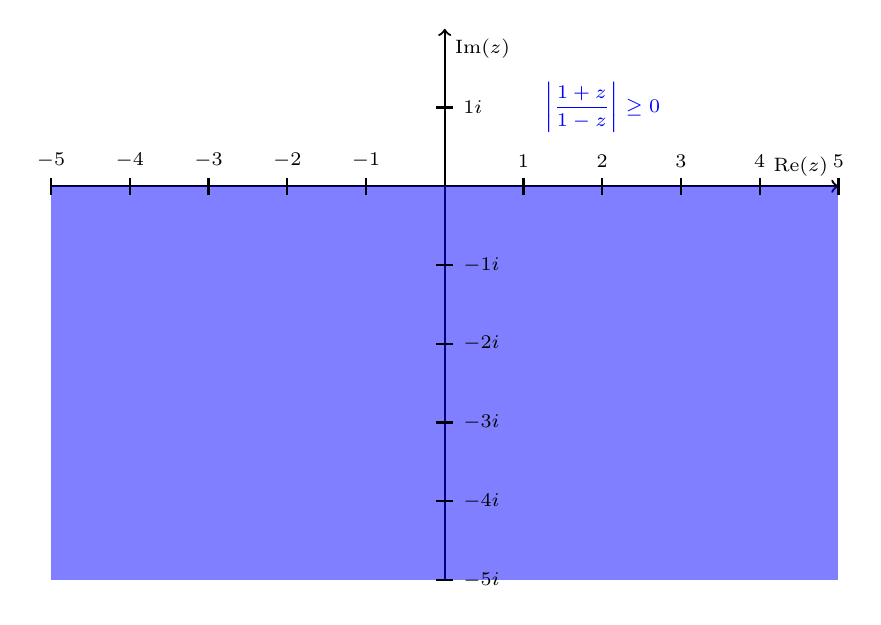
\begin{tikzpicture}
    \begin{scope}[thick,font=\scriptsize]

        \draw [->] (-5,0) -- (5,0) node [above left]  {Re$(z)$};
        \draw [->] (0,-5) -- (0,2) node [below right] {Im$(z)$};

        \path [draw=none,fill=blue,opacity = 0.5] (-5,-5) rectangle (5,0);

        \foreach \n in {-5,...,-2,-1,1}{%
            \draw (\n,-3pt) -- (\n,3pt)   node [above] {$\n$};
            \draw (-3pt,\n) -- (3pt,\n)   node [right] {$\n i$};
        }
            \draw (2,-3pt) -- (2,3pt)   node [above] {$2$};
            \draw (3,-3pt) -- (3,3pt)   node [above] {$3$};
            \draw (4,-3pt) -- (4,3pt)   node [above] {$4$};
            \draw (5,-3pt) -- (5,3pt)   node [above] {$5$};

        \node [color=blue] at (2,1) {$\displaystyle\left|\frac{1+z}{1-z}\right| \geq 0$};
    \end{scope}

\end{tikzpicture}
\end{document}
